
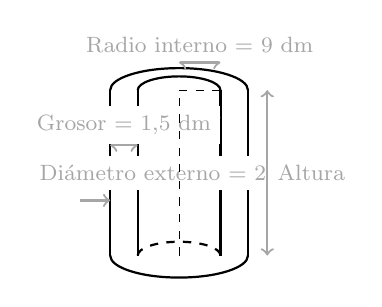
\begin{tikzpicture}[scale=0.7]
  % Definir estilos
  \tikzset{
    linea_medida/.style={gray!70, thick, <->},
    flecha_linea/.style={->, thick, gray!70},
    etiqueta/.style={fill=white, font=\footnotesize}
  }

  % Cilindro externo - parte frontal visible
  \draw[thick] (-1.25,0) arc (180:360:1.25cm and 0.4cm);
  \draw[thick] (-1.25,3) arc (180:0:1.25cm and 0.4cm);
  \draw[thick] (-1.25,0) -- (-1.25,3);
  \draw[thick] (1.25,0) -- (1.25,3);

  % Cilindro interno - parte frontal visible
  \draw[thick, dashed] (-0.75,0) arc (180:0:0.75cm and 0.25cm);
  \draw[thick] (-0.75,3) arc (180:0:0.75cm and 0.25cm);
  \draw[thick] (-0.75,0) -- (-0.75,3);
  \draw[thick] (0.75,0) -- (0.75,3);

  % Líneas de medida
  \draw[linea_medida] (-2,1.5) -- (2,1.5) node[midway, etiqueta] {Diámetro externo =  21   dm };
  \draw[linea_medida] (0,3.5) -- (0.75,3.5) node[midway, etiqueta, above] {Radio interno =  9   dm };

  % Línea de altura
  \draw[linea_medida] (1.6,0) -- (1.6,3) node[midway, etiqueta, right] {Altura};

  % Etiqueta de radio interno
  \draw[flecha_linea] (0.2,2.5) -- (0,2.5);
  \draw[flecha_linea] (0.2,2.5) -- (0.75,2.5);

  % Etiqueta de radio externo
  \draw[flecha_linea] (-1.8,1) -- (-1.25,1);

  % Etiqueta de grosor
  \draw[linea_medida] (-1.25,2) -- (-0.75,2) node[midway, etiqueta, above] {Grosor =  1,5   dm };

  % Líneas punteadas para ilustrar dimensiones
  \draw[dashed] (0,3) -- (0.75,3);
  \draw[dashed] (0,0) -- (0,3);
\end{tikzpicture}
